\subsection{Our classifiers} \label{supervised_approach_models}

We implement the convolutional neural network detailed in \cite{gargiulo2019deep}, as their use case closely resembles ours (see section \ref{hmc_gargiulo}). They also work with scientific texts and assign to them subjects organized in a hierarchy. The paper provides a complete architecture, from processing the text, to extracting features and feeding them to a classifier. Their architecture is grounded on previous work, which makes their design decisions more sound. Our use cases differ mainly in three points:

\begin{enumerate}
    \item \textbf{Training data}: they have over eleven million documents, two orders of magnitude more than us.
    \item \textbf{Label noise}: their subject indexing procedure was performed by humans, whereas ours was performed by an unsupervised algorithm, which is not as accurate.
    \item \textbf{Subject hierarchy}: theirs comprises more than 20,000 subjects, one order of magnitude more than us.
\end{enumerate}

We consider these differences when adapting the architecture for our case. We discuss the design choices of the original architecture and the changes we have made in section \ref{supervised_approach_design}. These include reducing the size of the model, given our smaller number of labels and our shorter inputs, increasing the dropout probability, which was very low in the original implementation, and using a learning rate schedule instead of keeping it constant.

In section \ref{supervised_approach_add_asymmetry}, we replace the loss function of our model with one specifically designed for \acrfull{mlc} \cite{ben2020asymmetric} that decouples positive from negative labels, which allows the model to focus on the rare positive samples instead of on the numerous negative ones. See section \ref{hmc_asl} for more details. This loss function was used in \cite{zhao2021evaluating} to evaluate \acrshort{mlc} with noisy labels, concluding that it increased the regularization of the model, thus avoiding overfitting the noisy data. Therefore, this loss function may help us address label noise, the second difference between the original use case and ours.

The second extension we implement is the addition of the \acrlong{mcm} and using the \acrfull{mcl} \cite{giunchiglia2020coherent} as our model's loss function. To the best of our knowledge, it is the current \acrshort{sota} for \acrshort{hmc}. The paper was already presented in section \ref{hmc_forward}. Given that both the \acrshort{asl} and the \acrshort{mcl} extend the \acrshort{bce}, we combine them, yielding the \acrlong{aml}, which we use for this model.

We thus have three models. They only differ on the loss function, and the additional layer of the coherent model. All other model parameters, as well as the training settings, are the same. For brevity, we refer to each of the three models by their loss function: the \acrshort{bce} model, the \acrshort{asl} model and the \acrshort{aml} model. We present their architecture and parameters in the following sections.

\subsubsection{Design of the classifying pipeline} \label{supervised_approach_design}

\begin{figure}
    \centering
    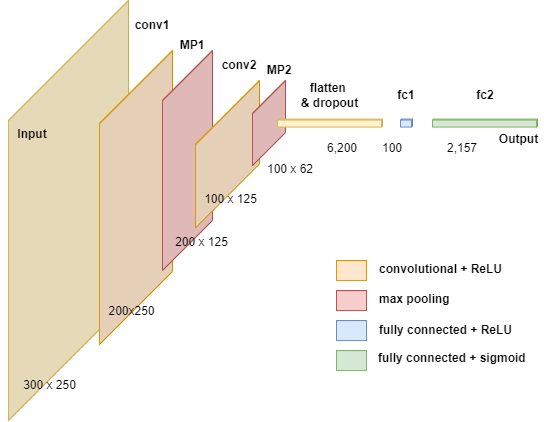
\includegraphics[width=.85\textwidth]{figures/supervised_approach/model_diagram.png}
    \caption{Diagram of the model. The shown sizes are the outputs of each layer.}
    \label{fig:model_diagram}
\end{figure}

Our model comprises two phases: one where feature extraction is performed, and a second one where the probabilities of each subject being assigned to the input document are computed. We first define the input to the model, which is not the same as for the original implementation (i.e. the one from \cite{gargiulo2019deep}), given our different use cases. We use only one representation type instead of four, and we keep the first 250 words of each text, instead of the first 400. Then, we explain the architecture of the model. We adapt the original implementation to our use case, and also optimize several aspects through experimentation. Please note that a description of how convolutions are applied to text was given in section \ref{hmc_cnn}.

\paragraph{Input} \mbox{}

The input to the model is a collection of word vectors. In the original implementation, they pick the first 400 words of each text and discard the rest. If a text has less than 400 words, they pad it with zero vectors. As shown in figure \ref{fig:sm_doc_length}, most of our documents have less than 250 tokens. We therefore pick 250 as our threshold, and also pad when necessary. Some representations are very short because the documents don't have abstracts, or because they are written in other languages and tagged as they were in English (see section \ref{repo_analysis_data}).

We only consider the tokens for which we have a pre-trained vector. The fastText word vectors are 300-dimensional, meaning they comprise 300 floating numbers each. Thus, the input is formed by 250 word vectors, each with 300 dimensions. As shown in figure \ref{fig:model_diagram}, the input forms a matrix, where each word vector is a column.

\begin{figure}
    \centering
    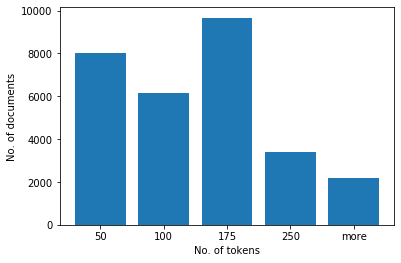
\includegraphics[width=.6\textwidth]{figures/supervised_approach/sm_doc_length.png}
    \caption{No. of tokens per document, in five groups.}
    \label{fig:sm_doc_length}
\end{figure}

\paragraph{Model architecture} \mbox{}

The feature extraction phase comprises two convolutional layers, each followed by ReLU activation and a max-pooling layer. Both pooling layers have a kernel size of 2, and both convolutional layers have stride 1. The stride defines the steps taken across the input between convolutions. Furthermore, both convolutional layers use padding to keep the number of dimensions unaltered

The first convolutional layer has 200 filters and kernel size 5. The number of filters is the number of features extracted from the input. Thus, the resulting matrix has 200 rows and the same number of columns, as shown in figure \ref{fig:model_diagram} in the \textit{conv1} layer. The kernel size defines how large a context window should be considered for each word vector. The second convolutional layer has 100 filters and kernel size 3. The resulting matrix, which comprises 100 rows and 62 columns, is flattened into a one-dimensional vector. Then, its constituent elements are zeroed with a certain dropout probability, a regularization technique used to avoid overfitting. The probability of this layer is discussed in the following section.

The assignment probabilities for each document are computed by a classifier consisting of two fully connected layers. The size of the output is equivalent to the number of subjects, as we want to output an assignment probability for each of them. The output layer also has sigmoid activation instead of ReLU, so each probability is between zero and one. The size of the first layer, called the hidden layer, comprises 1,024 neurons in the original paper, as their number of subjects exceeds 20,000. Given that our set of subjects is one order of magnitude smaller, we have reduced the size of the hidden layer. We experiment with 100 and 200 neurons in appendix \ref{supervised_approach_optim}. As both values perform similarly, we keep the lower one for further regularization and less computational cost.

\subsubsection{Training parameters} \label{supervised_approach_params}

The model parameters are optimized using \acrfull{sgd}, where the gradient is estimated by considering only a subset of the data. It is a trade-off between computational cost and fast convergence rate, parameterized by the batch size. A larger batch size accelerates convergence (regarding the number of steps), but also increases the computational cost. The original implementation uses a batch size of 10 and improve the convergence rate with a Nesterov momentum of $0.5$. Momentum introduces inertia into the gradient space, meaning that the direction of the steps are influenced by previous steps. They use \acrfull{bce} as a loss function. As discussed in section \ref{hmc_asl}, this is the common loss function for multi-label settings.

We experimented with two different sizes for the hidden layer: 100 and 200. The results showed that both sizes performed similarly. We decided to keep the lower size, which reduces the computational cost and increases regularization. We also experimented with two values for the dropout probability which were common in the literature: 30 \% and 70 \%, concluding that the higher value offers better results. The original implementation used a dropout probability of 10 \%, which is very low when compared with the literature. Both experiments can be found in appendix \ref{supervised_approach_optim}.

Interestingly, the original implementation doesn't use a learning rate (LR) scheduler, which is common practice in deep learning. Instead, they keep the LR constant at $0.1$. This is not optimal, both in terms of efficiency and accuracy. Gradient steps should be larger when further away from the optimum, to increase convergence rate, and decrease over time to not overshoot the optimum. Our experiments, presented in appendix \ref{supervised_approach_optim}, show that the 1-cycle policy fits our use case better than a decaying LR schedule. Cyclical LR schedules \cite{smith2017cyclical} follow the observation that increasing the LR may lead the model to perform better in the long term. The 1-cycle policy increases the LR until it reaches a given maximum, and then decreases it monotonically afterwards.

\subsubsection{Adding asymmetry} \label{supervised_approach_add_asymmetry}

Our first extension of the model described above, which we term \acrshort{bce} model because of its loss function, is to replace its loss function with the \acrfull{asl}, resulting in the \acrshort{asl} model. The \acrshort{asl}, which was already presented in section \ref{hmc_asl}, extends the \acrfull{bce} loss to address the imbalance between positive and negative samples in multi-label settings. It receives two parameters, $\gamma_-$ and $\gamma_+$. They modulate the importance of negative and positive samples, respectively. The larger their values, the lower the impact of their corresponding samples on the result of \acrshort{asl}.

We have experimented with these parameters in appendix \ref{supervised_approach_asymmetric}, concluding that the optimal values for our use case are $\gamma_+=1$ and $\gamma_-=2$. Recall that the \acrshort{asl} model is exactly the same as the \acrshort{bce} model, except for the loss function.

\subsubsection{Adding coherence} \label{supervised_approach_add_coherence}

The second extension of the \acrshort{bce} model is the addition of a new layer, called the \acrfull{mcm}, and the use of the \acrfull{aml}. The \acrshort{mcm}, which was presented in section \ref{hmc_forward}, enforces the subject hierarchy upon the output of the model, so subjects have an assignment probability at least as high as the assignment probabilities of their descendants. In practice, the \acrshort{mcm} is implemented as a matrix, where each row has ones for the subject it represents and its descendants, and zeros otherwise. Each row of this matrix is multiplied element-wise with the output of the model. Then, the maximum of each row is assigned to the corresponding subject.

The loss function used by the original coherent model \cite{giunchiglia2020coherent}, called the \acrfull{mcl}, modifies \acrshort{bce} loss to also ensure that the assignment probabilities respect the subject hierarchy. Given that the \acrshort{asl} also extends  \acrshort{bce}, we can combine them. Below is a comparison of all three loss functions, and their resulting combination, which we term \acrfull{aml}. In these formulas, $D(x)$ is the set of subjects that are descendants of subject $x$. All the individual losses are then averaged to arrive at the final loss for a document, which has as many of these input-output pairs as there are subjects.

\begin{align*}
    & BCE(x, y) = -y \cdot \log (x) - (1-y) \cdot \log (1-x) \\ \\
    & ASL_{\gamma_-, \gamma_+}(x, y) = -y \cdot \log (p) \cdot (1-p)^{\gamma_+} - (1-y) \cdot \log (1-p) \cdot p^{\gamma_-} \\ \\
    & MCL(x, y) = -y \cdot \log (\max(x, \{x_d \cdot y_d, \forall d \in D(x)\}) - (1 - y) \cdot \log (1 - MCM_x) \\ \\
    & AML_{\gamma_-, \gamma_+}(x, y) = -y \cdot \log (\max(x, \{x_d \cdot y_d, \forall d \in D(x)\}) \cdot (1-p)^{\gamma_+} \\
    & \qquad \qquad \qquad \qquad - (1 - y) \cdot \log (1 - MCM_x) \cdot p^{\gamma_-} \\
\end{align*}

We have performed an experiment to compare the \acrshort{mcl} with the \acrshort{aml}, outlined in appendix \ref{supervised_approach_coherence}, concluding that \acrshort{aml} performs better in our dataset. We thus use the \acrshort{aml} in our third supervised model.